\documentclass[a4paper]{article}
\usepackage[margin=15mm]{geometry}
\usepackage{tikz}
\usetikzlibrary{calc}
\usetikzlibrary{arrows.meta}
\usetikzlibrary{patterns}

\begin{document}

% ============================================
% PARAMETER DEFINITIONS
% ============================================
\def\scalefactor{0.13}  % Scale factor for drawing (increased from 0.10)

% Shaft dimensions
\def\Do{38}             % Shaft outer diameter [mm]

% Beam dimensions
\def\beamwidth{2}       % Beam width (y-direction) [mm]
\def\clampheight{10}    % Clamp height [mm]

% Bending deformation parameters
\def\Lin{900}           % Inboard length [mm]
\def\wmax{50}           % Maximum deflection [mm]
\def\xb{200}            % Beam root position [mm]
\def\Lb{100}            % Beam length [mm]

% Beam offset
\pgfmathsetmacro{\ybeam}{\Do/2 + \clampheight}

% ============================================
% MAIN BENDING VIEW
% ============================================
\begin{center}
\begin{tikzpicture}[x=\scalefactor mm, y=\scalefactor mm, 
    declare function={
        w(\x) = -50 * (\x/900) * (\x/900) * (3 - 2*\x/900);
    }]

% Title
\node[anchor=south, font=\Large\bfseries] at (450, 100) {Inboard Shaft Bending - Top View (Exaggerated)};

% Shaft centerline  
\draw[thick, gray!60, dashed] plot[domain=0:900, samples=50] (\x, {w(\x)});

% Shaft
\draw[thick, black, fill=gray!30] 
    plot[domain=0:900, samples=50] (\x, {w(\x) + 19})
    -- plot[domain=900:0, samples=50] (\x, {w(\x) - 19})
    -- cycle;

% Beam
\draw[thick, green!60!black, fill=green!20] 
    plot[domain=200:300, samples=25] (\x, {w(\x) + 29 + 1})
    -- plot[domain=300:200, samples=25] (\x, {w(\x) + 29 - 1})
    -- cycle;

% Clamps
\draw[thick, green!60!black] (200, {w(200) + 19}) -- (200, {w(200) + 28});
\draw[thick, green!60!black] (300, {w(300) + 19}) -- (300, {w(300) + 28});

% Fixed support at x=0
\draw[pattern=north east lines, pattern color=black] 
    (-20, -20) rectangle (0, 45);
\draw[very thick] (0, -20) -- (0, 45);

% Applied force at handle
\draw[->, >=latex, line width=2pt, blue!70!black] 
    (900, {w(900)}) -- (900, {w(900) - 200})
    node[right, font=\bfseries] {$F$};

% Axes
\draw[->, >=Stealth, thick, gray] (-50, 0) -- (950, 0) node[right] {$x$};
\draw[->, >=Stealth, thick, gray] (0, -80) -- (0, 100) node[above] {$y$};

% Position markers
\draw[thick] (0, -5) -- (0, 5);
\node[anchor=north, font=\small] at (0, -10) {$0$};

\draw[thick] (900, -5) -- (900, 5);
\node[anchor=north, font=\small] at (900, -10) {$x_F$};

\draw[thick] (200, -5) -- (200, 5);
\node[anchor=north, font=\small] at (200, -10) {$x_b$};

\draw[thick] (300, -5) -- (300, 5);
\node[anchor=north, font=\small] at (300, -10) {$x_b+L_b$};

% Deflection annotation
\draw[<->, >=Stealth, thick, red] 
    (920, 0) -- (920, {w(900)})
    node[midway, right, font=\small] {$w_{max}$};

% Zoom box indication
\draw[dashed, red, thick] (150, {w(200) - 30}) rectangle (350, {w(250) + 40});
\node[anchor=south west, font=\small, red] at (150, {w(250) + 40}) {Zoomed view below};

\end{tikzpicture}
\end{center}

\vspace{10mm}

% ============================================
% ZOOMED VIEW OF BEAM REGION
% ============================================
\begin{center}
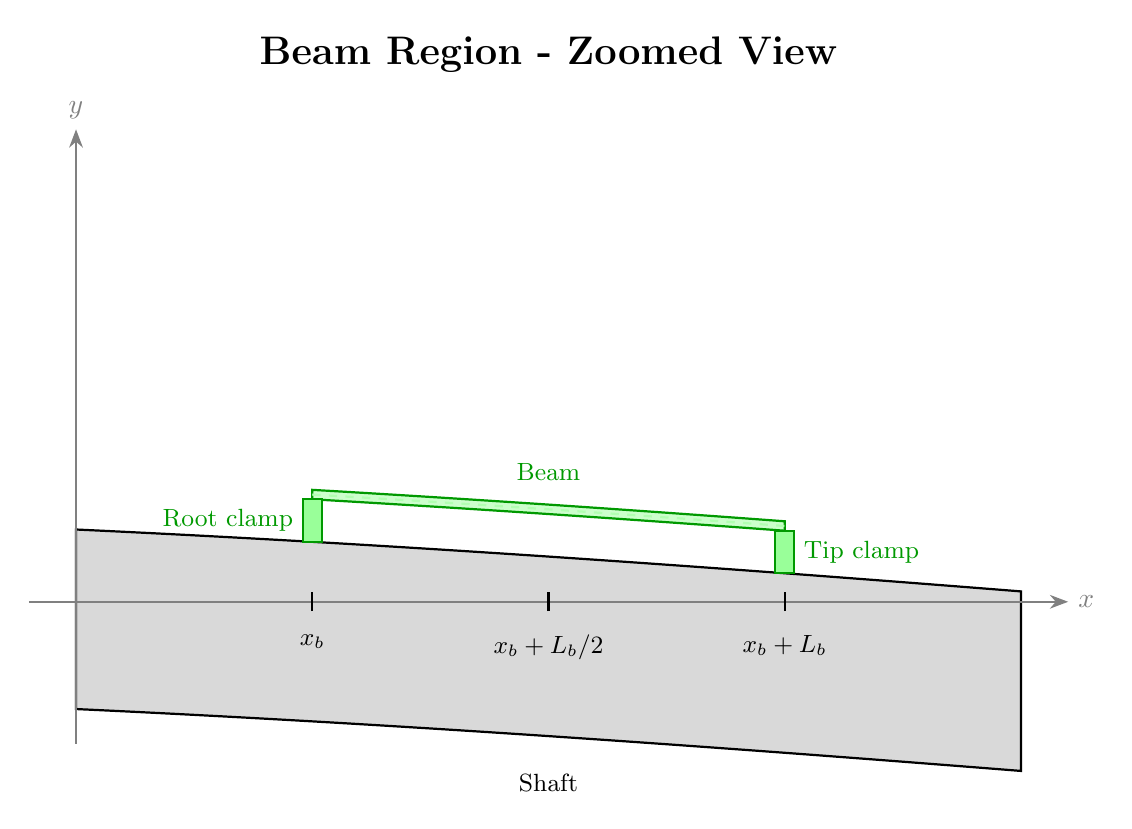
\begin{tikzpicture}[x=0.6mm, y=0.6mm, 
    declare function={
        w(\x) = -50 * (\x/900) * (\x/900) * (3 - 2*\x/900);
    }]

% Title
\node[anchor=south, font=\Large\bfseries] at (250, 110) {Beam Region - Zoomed View};

% Shaft centerline  
\draw[thick, gray!60, dashed] plot[domain=150:350, samples=50] (\x, {w(\x)});

% Shaft
\draw[thick, black, fill=gray!30] 
    plot[domain=150:350, samples=50] (\x, {w(\x) + 19})
    -- plot[domain=350:150, samples=50] (\x, {w(\x) - 19})
    -- cycle;

% Beam
\draw[thick, green!60!black, fill=green!20] 
    plot[domain=200:300, samples=25] (\x, {w(\x) + 29 + 1})
    -- plot[domain=300:200, samples=25] (\x, {w(\x) + 29 - 1})
    -- cycle;

% Beam centerline
\draw[thick, green!30, dashed] plot[domain=200:300, samples=25] (\x, {w(\x) + 29});

% Clamps (detailed)
\draw[thick, green!60!black] (200, {w(200) + 19}) -- (200, {w(200) + 28});
\draw[thick, green!60!black] (300, {w(300) + 19}) -- (300, {w(300) + 28});

% Clamp rectangles for better visualization
\draw[thick, green!60!black, fill=green!40] 
    (198, {w(200) + 19}) rectangle (202, {w(200) + 28});
\draw[thick, green!60!black, fill=green!40] 
    (298, {w(300) + 19}) rectangle (302, {w(300) + 28});

% Axes
\draw[->, >=Stealth, thick, gray] (140, 0) -- (360, 0) node[right] {$x$};
\draw[->, >=Stealth, thick, gray] (150, -30) -- (150, 100) node[above] {$y$};

% Position markers
\draw[thick] (200, -2) -- (200, 2);
\node[anchor=north, font=\small] at (200, -5) {$x_b$};

\draw[thick] (300, -2) -- (300, 2);
\node[anchor=north, font=\small] at (300, -5) {$x_b+L_b$};

\draw[thick] (250, -2) -- (250, 2);
\node[anchor=north, font=\small] at (250, -5) {$x_b + L_b/2$};

% Labels
\node[anchor=north, font=\small] at (250, {w(250) - 25}) {Shaft};
\node[anchor=south, font=\small, green!60!black] at (250, {w(250) + 33}) {Beam};
\node[anchor=east, font=\small, green!60!black] at (198, {w(200) + 23.5}) {Root clamp};
\node[anchor=west, font=\small, green!60!black] at (302, {w(300) + 23.5}) {Tip clamp};

% Dimension annotations
% \draw[<-, >=Stealth, thick, blue] 
%     (300, {w(250) + 29 - 1}) -- (300, {w(250) + 29 + 1})
%     node[midway, right, font=\small] {$w_b$};

% \draw[<-, >=Stealth, thick, red] 
%     (300, {w(250) +5 - 1}) -- (300, {w(250) +5 + 1})
%     node[midway, right, font=\small] {$w_s$};

% \draw[<->, >=Stealth, thick, orange] 
%     (360, {w(250) + 19}) -- (360, {w(250) + 28})
%     node[midway, right, font=\small] {$h_{clamp}$};

\end{tikzpicture}
\end{center}

\vspace{5mm}
\noindent\textbf{Author:} Sylvain Boyer (Mecafrog.com)

\end{document}